\chapter*{Tutorial Pembuatan Aplikasi Oracle Apex}

\begin{enumerate}
	\item Pertama buka link apex onlinenya yaitu  https://apex.oracle.com

	\item Setelah masuk ke web apexnya, lalu klik request a free workspace 
    \begin{figure}[!htbp]
    \begin{center}
    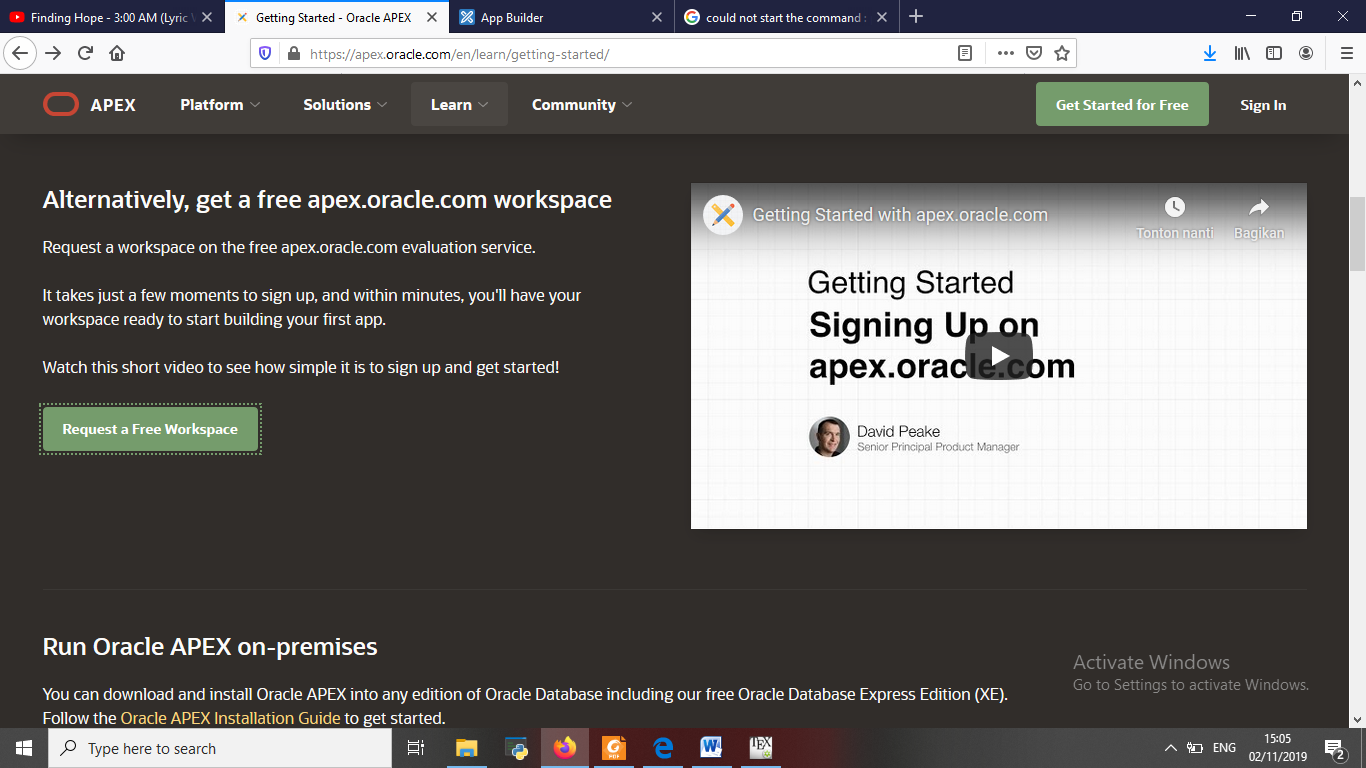
\includegraphics[scale=0.2]{Apex/0.png}
    \end{center}   
    \end{figure}
    
	\item Selanjutnya isi identificationnya, seperti gambar dibawah ini: 
	\begin{center}
    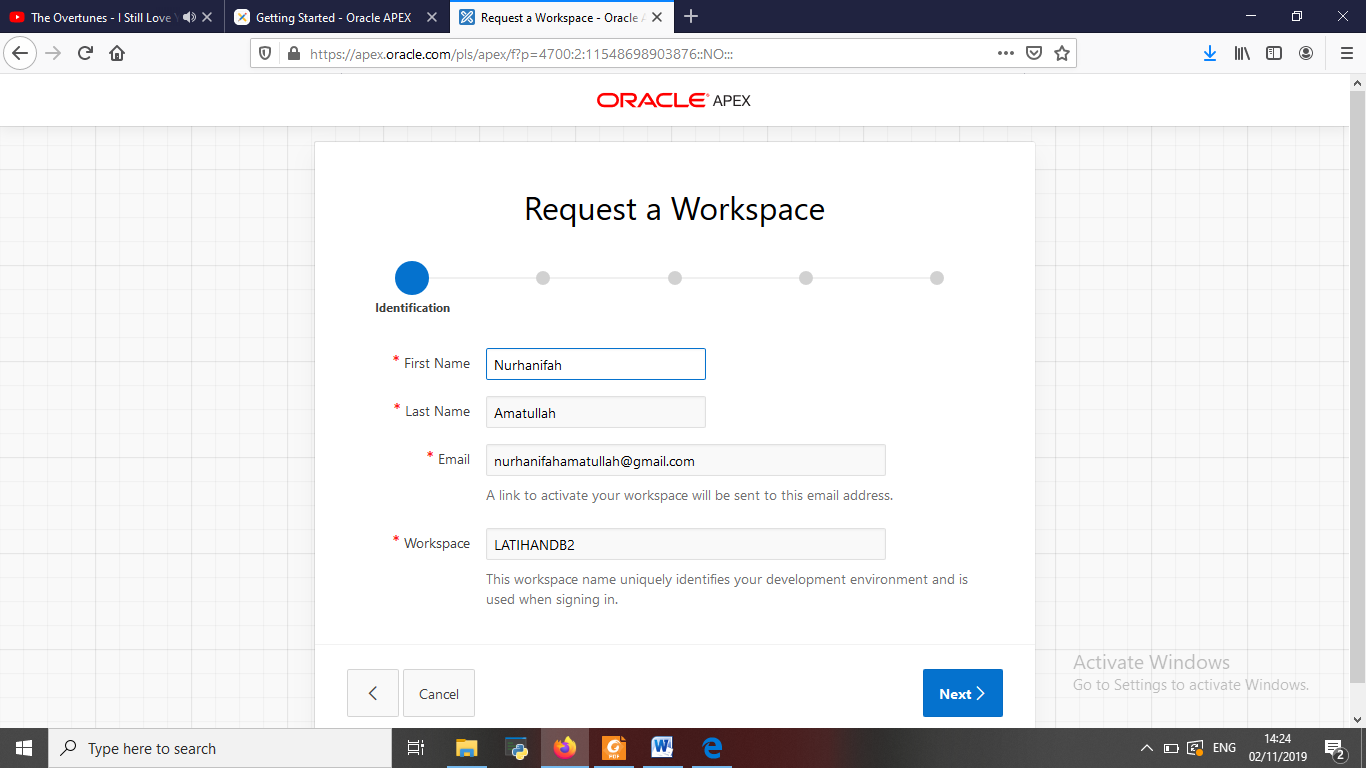
\includegraphics[scale=0.2]{Apex/1.png}
    \end{center}
    
	\item Setelah itu klik yes pada surveynya, dapat dilihat seperti dibawah ini:
	\begin{center}
    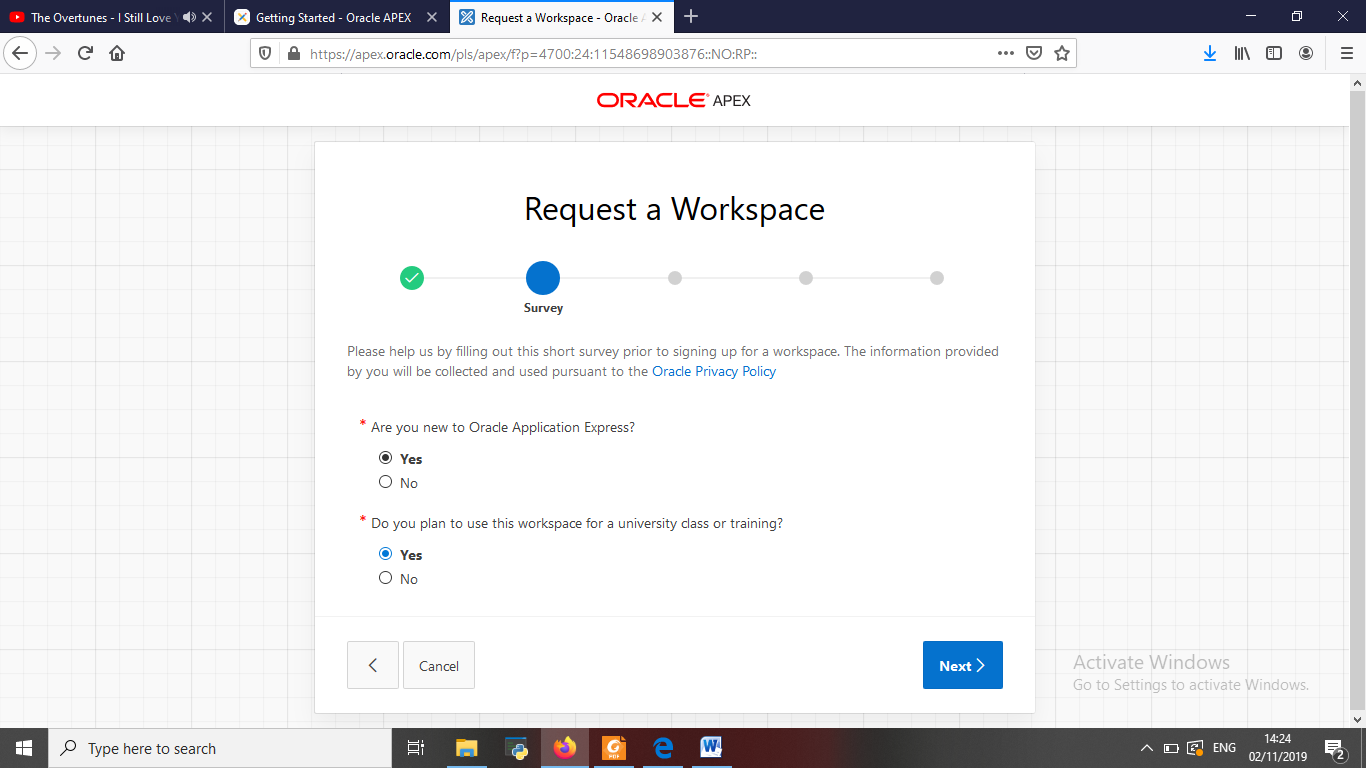
\includegraphics[scale=0.2]{Apex/2.png}
    \end{center}
	
	\item Lalu isi justificationnya 
	\begin{center}
    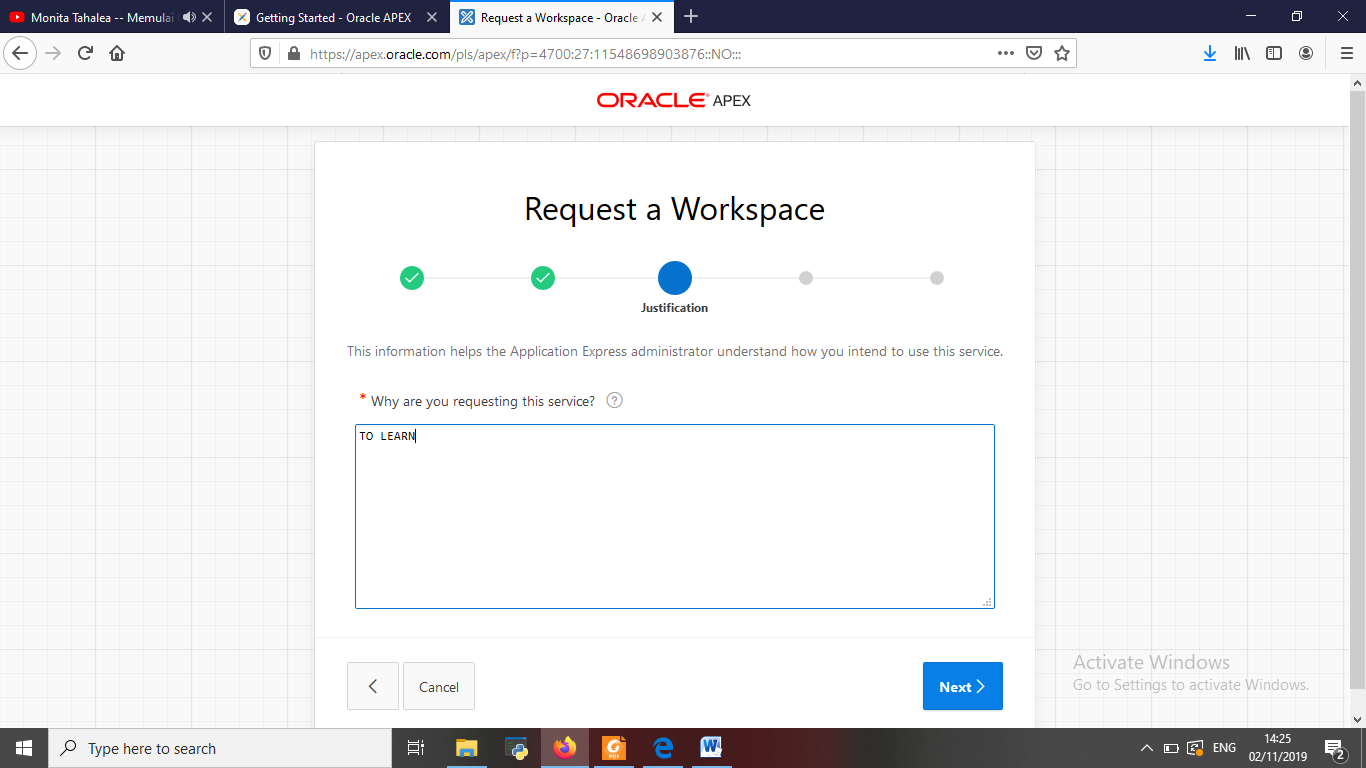
\includegraphics[scale=0.2]{Apex/3.png}
    \end{center}
    
	\item Kemudian centang I accept the terms pada agremeent
    \begin{center}
    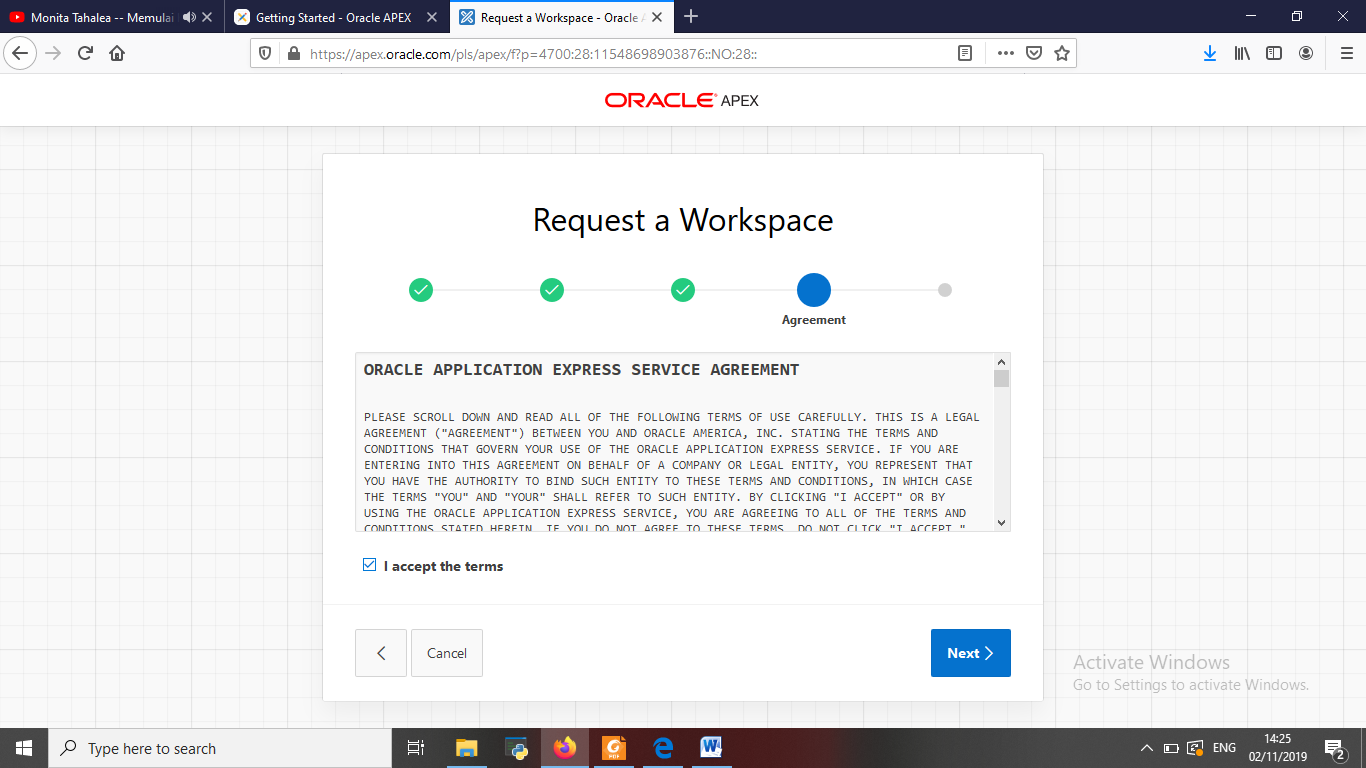
\includegraphics[scale=0.2]{Apex/4.png}
    \end{center}
	
	\item Setelah semuanya diisi, lalu pada bagian confirm klik submit request
	\begin{center}
    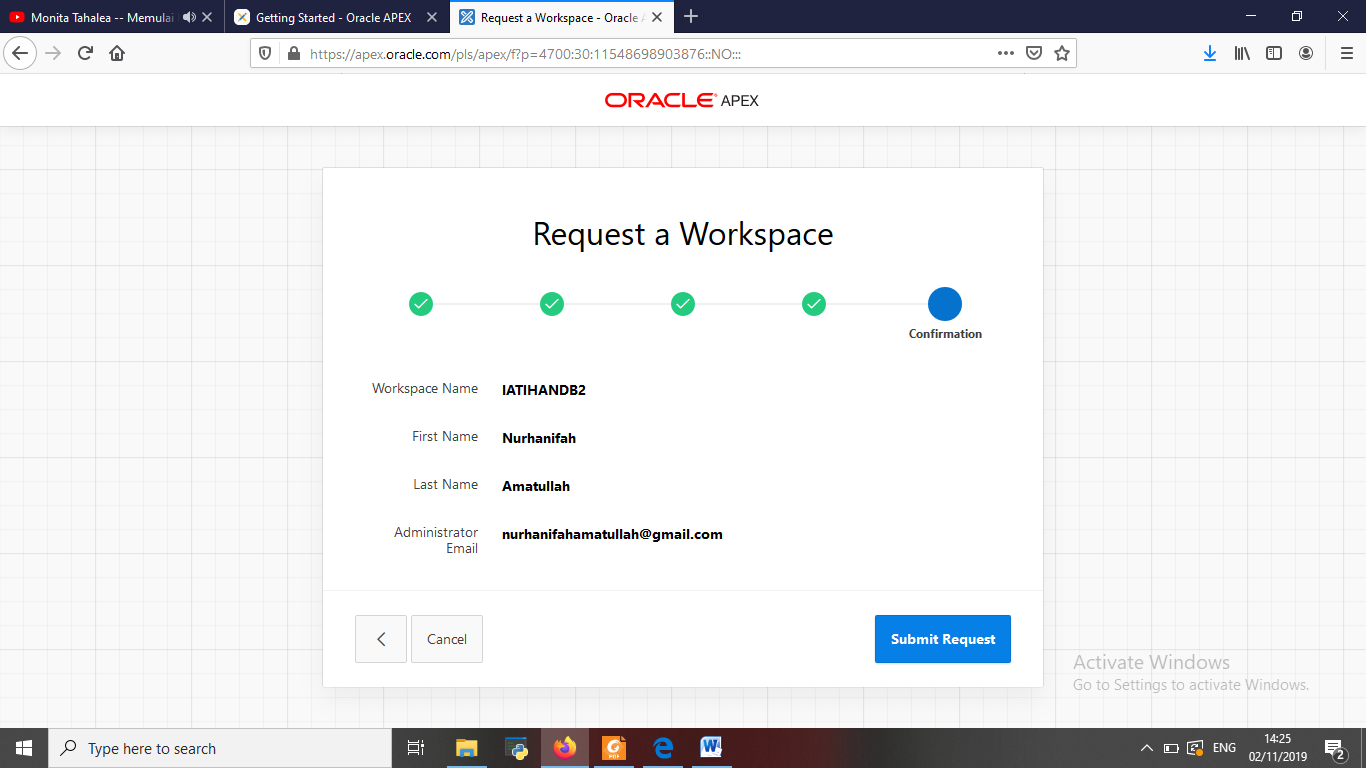
\includegraphics[scale=0.2]{Apex/5.png}
    \end{center}
	
	\item Selanjutnya buka email dan tunggu confirmasi diemail kita, lalu klik creat workspace 
	\begin{center}
    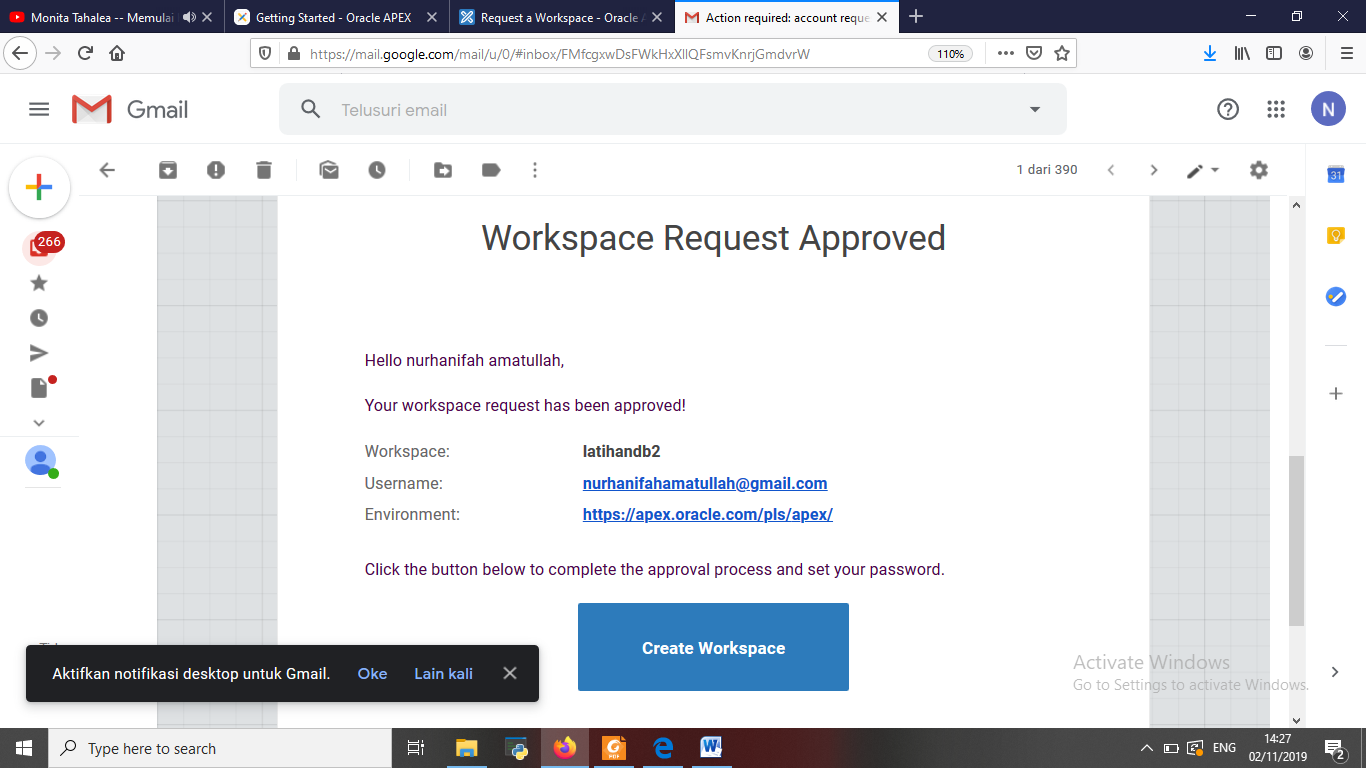
\includegraphics[scale=0.2]{Apex/6.png}
    \end{center}
	
	\item Lalu akan muncul Workspace Succesfully seperti gambar dibawah ini dan kllik continue to sign in screen
	\begin{center}
    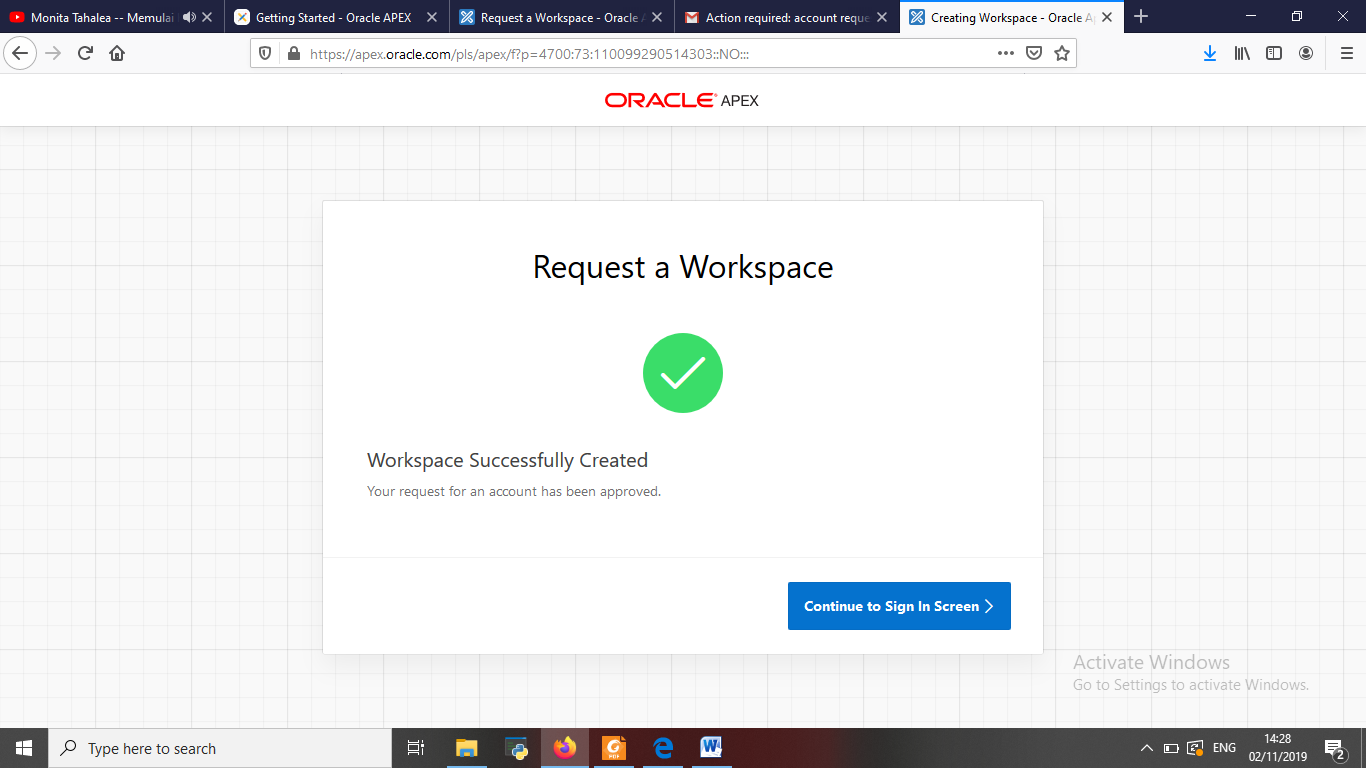
\includegraphics[scale=0.2]{Apex/7.png}
    \end{center}
	
	\item Setelah itu kita akan disuruh ganti password baru, seperti gambar dibawah ini
	\begin{center}
    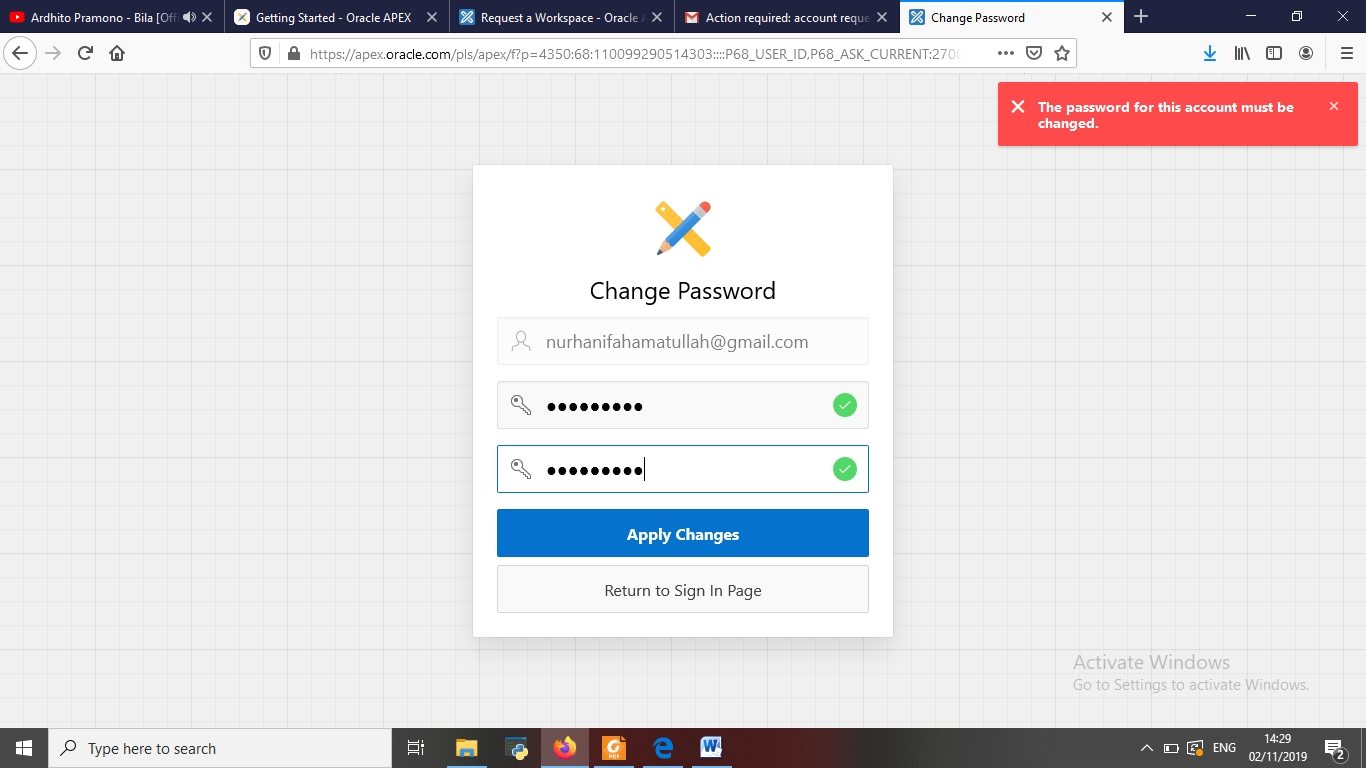
\includegraphics[scale=0.2]{Apex/8.png}
    \end{center}
	
	\item Kemudian setelah ganti password kita akan mucul ke halaman utama, Lalu klik app builder, dapat dilihat seperti gambar dibawah ini :
	\begin{center}
    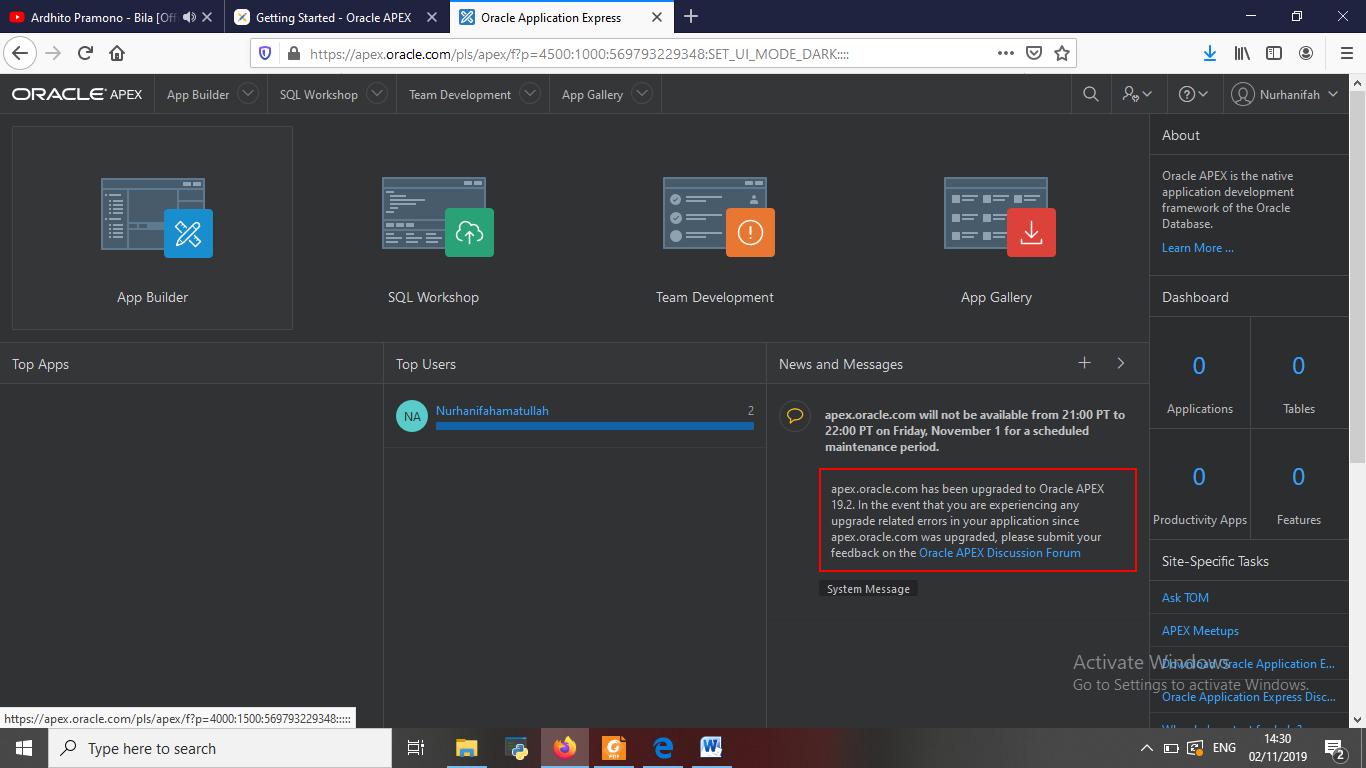
\includegraphics[scale=0.2]{Apex/9.png}
    \end{center}
	
	\item Selanjutnya klik create, seperti dibawah ini
	\begin{center}
    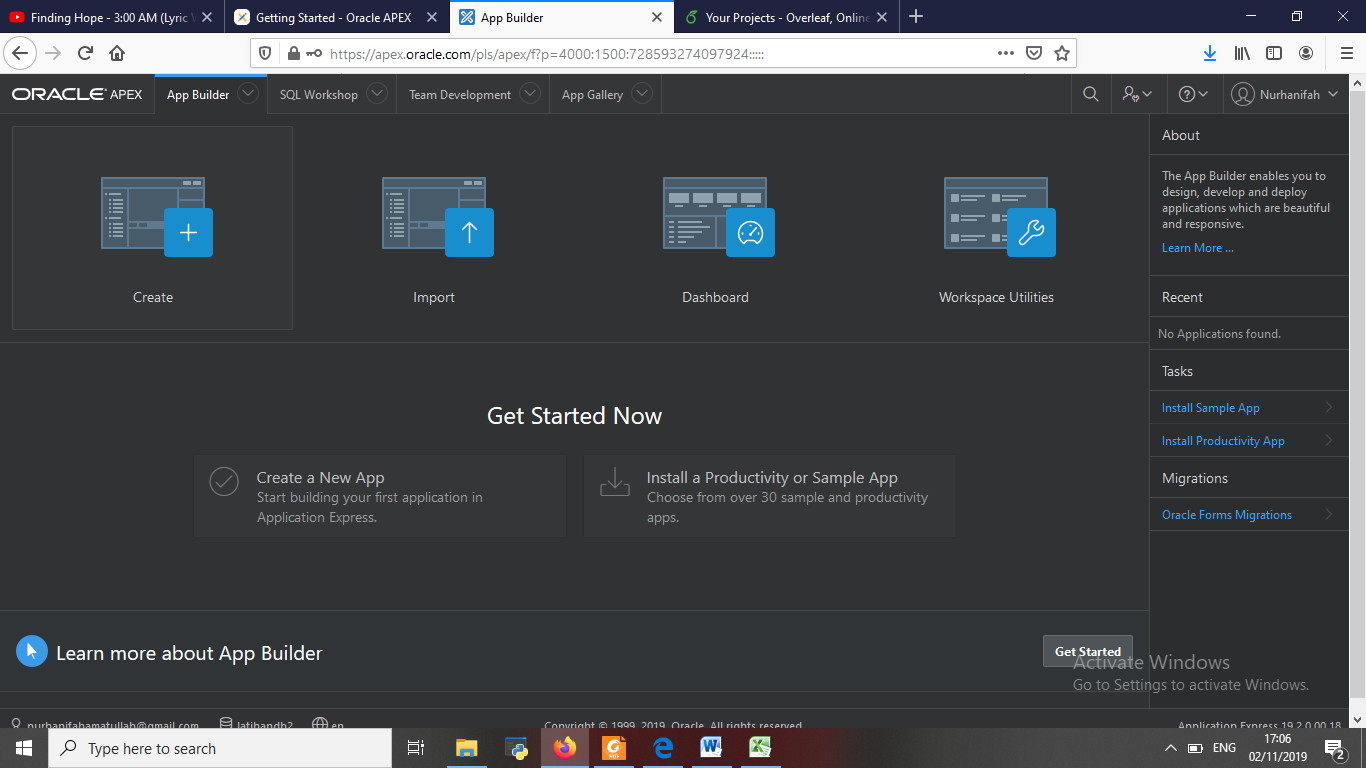
\includegraphics[scale=0.2]{Apex/10.png}
    \end{center}
    
	\item Lalu pilih form a file, seperti dibawah ini
	\begin{center}
    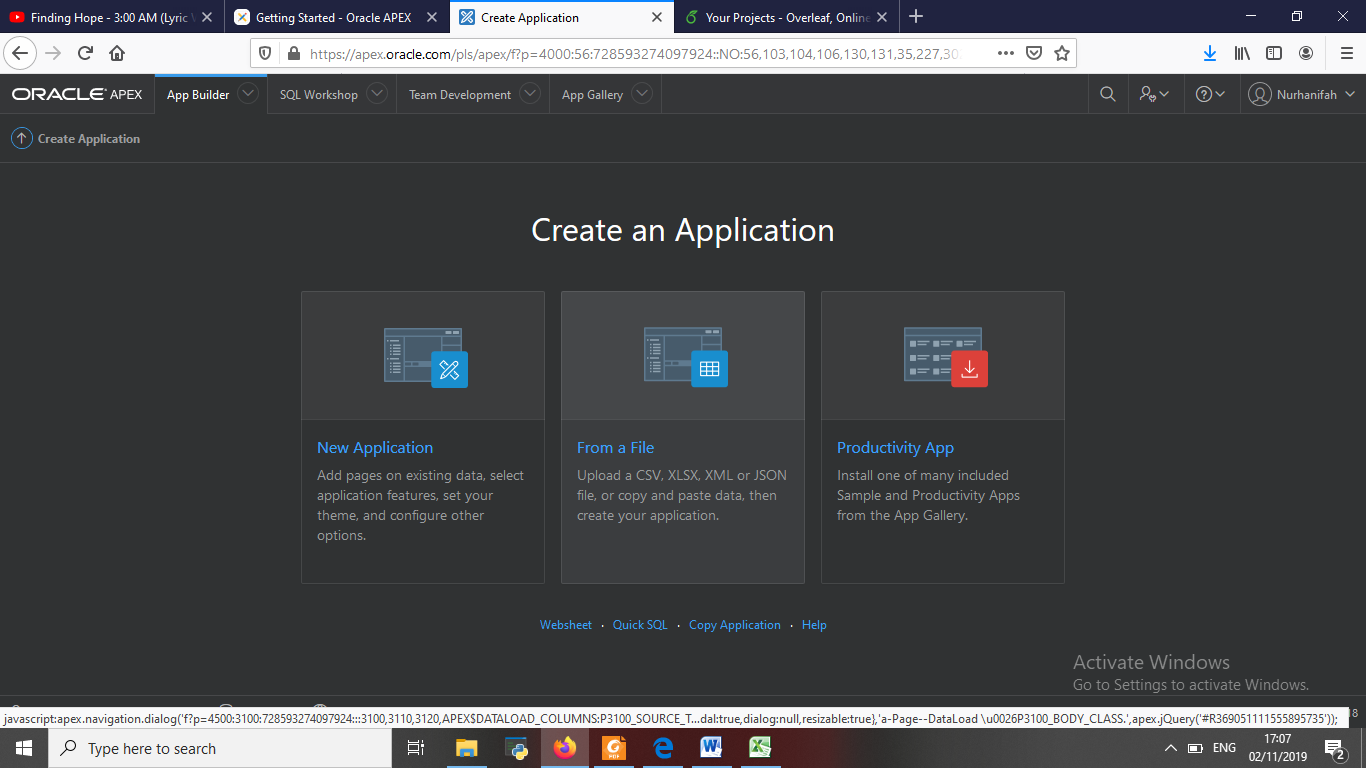
\includegraphics[scale=0.2]{Apex/11.png}
    \end{center}
    
    \item kemudian drag file yang sudah di export ke csv, seperti dibawah ini
	\begin{center}
    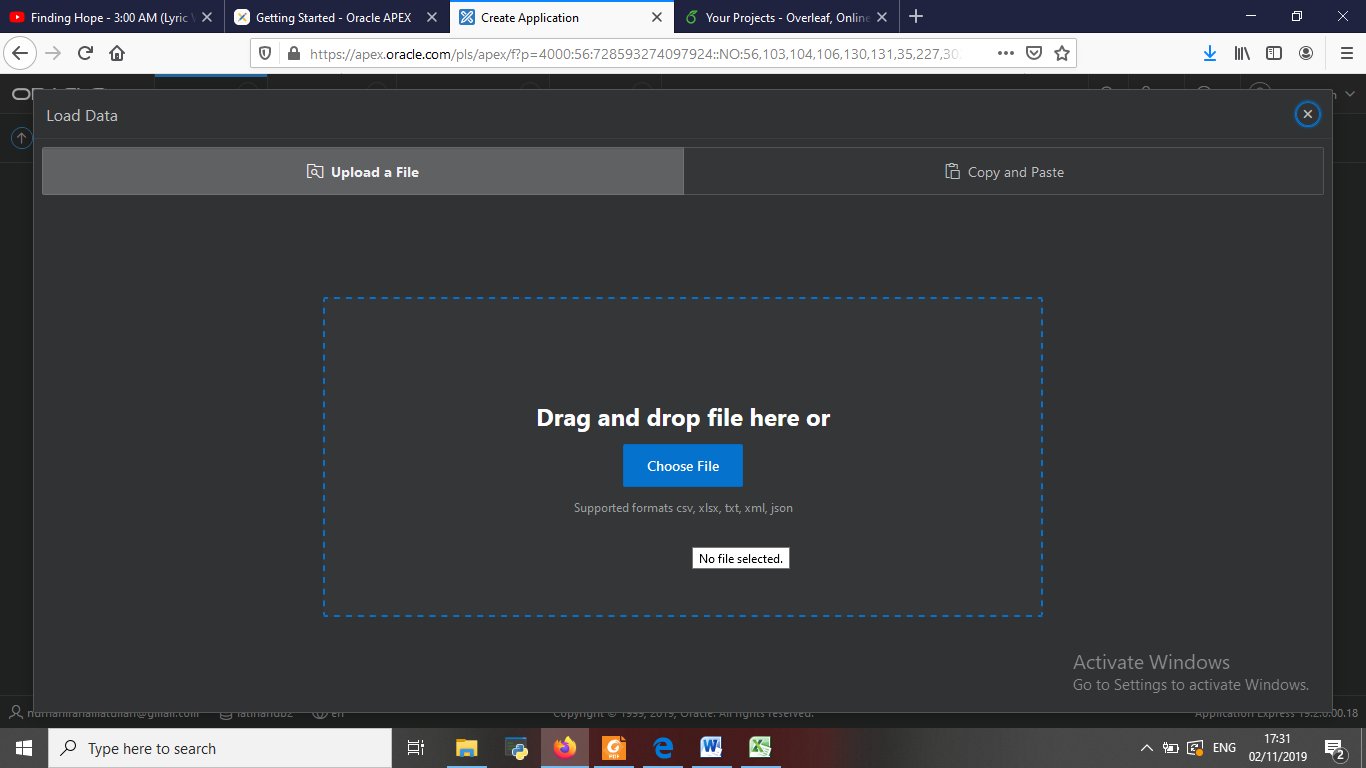
\includegraphics[scale=0.2]{Apex/12.png}
    \end{center}
    
    \item kemudian isi table name, seperti dibawah ini
	\begin{center}
    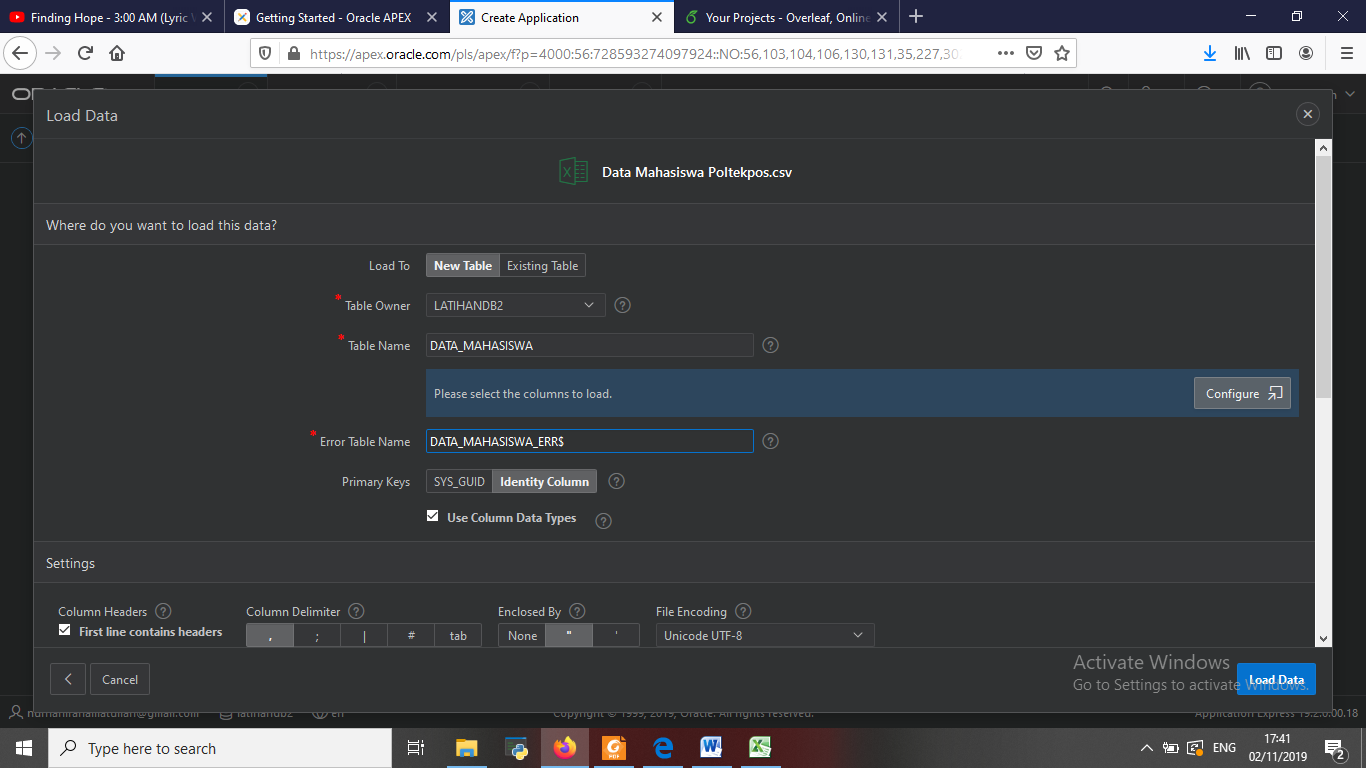
\includegraphics[scale=0.2]{Apex/13.png}
    \end{center}
    
    \item kemudian isi table name serta eror table name, Lalu klik load data, seperti dibawah ini
	\begin{center}
    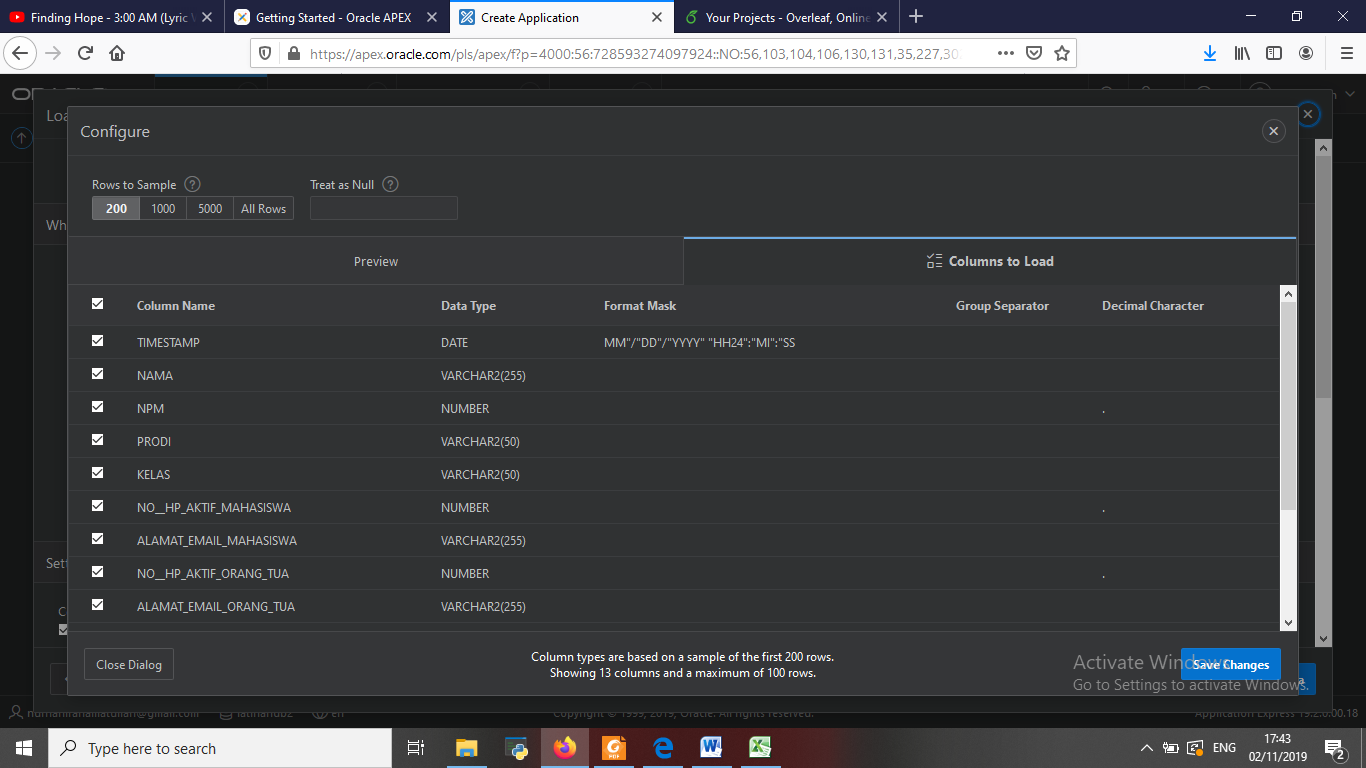
\includegraphics[scale=0.2]{Apex/14.png}
    \end{center}

    \item Setelah tampil seperti dibawah ini klik save changes
	\begin{center}
    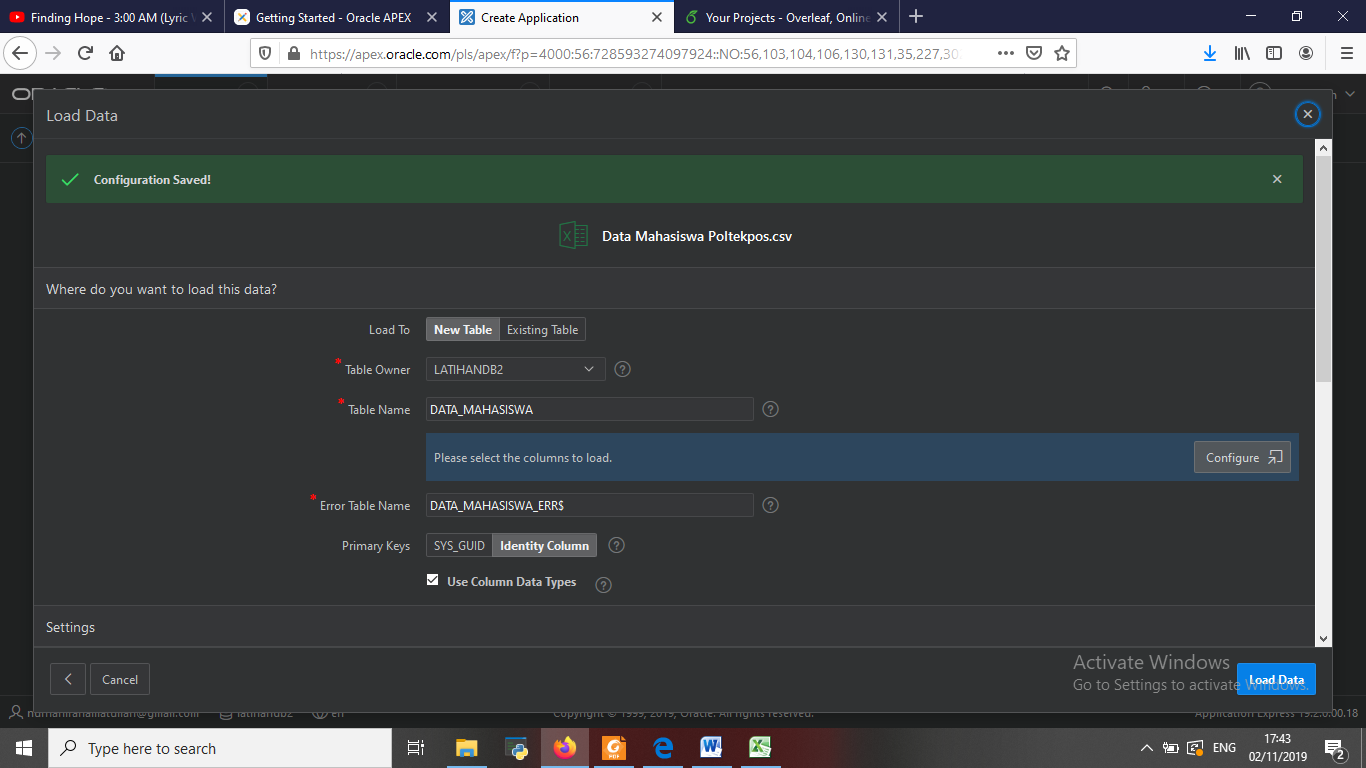
\includegraphics[scale=0.2]{Apex/15.png}
    \end{center}
    
    \item Setelah klik create aplication
	\begin{center}
    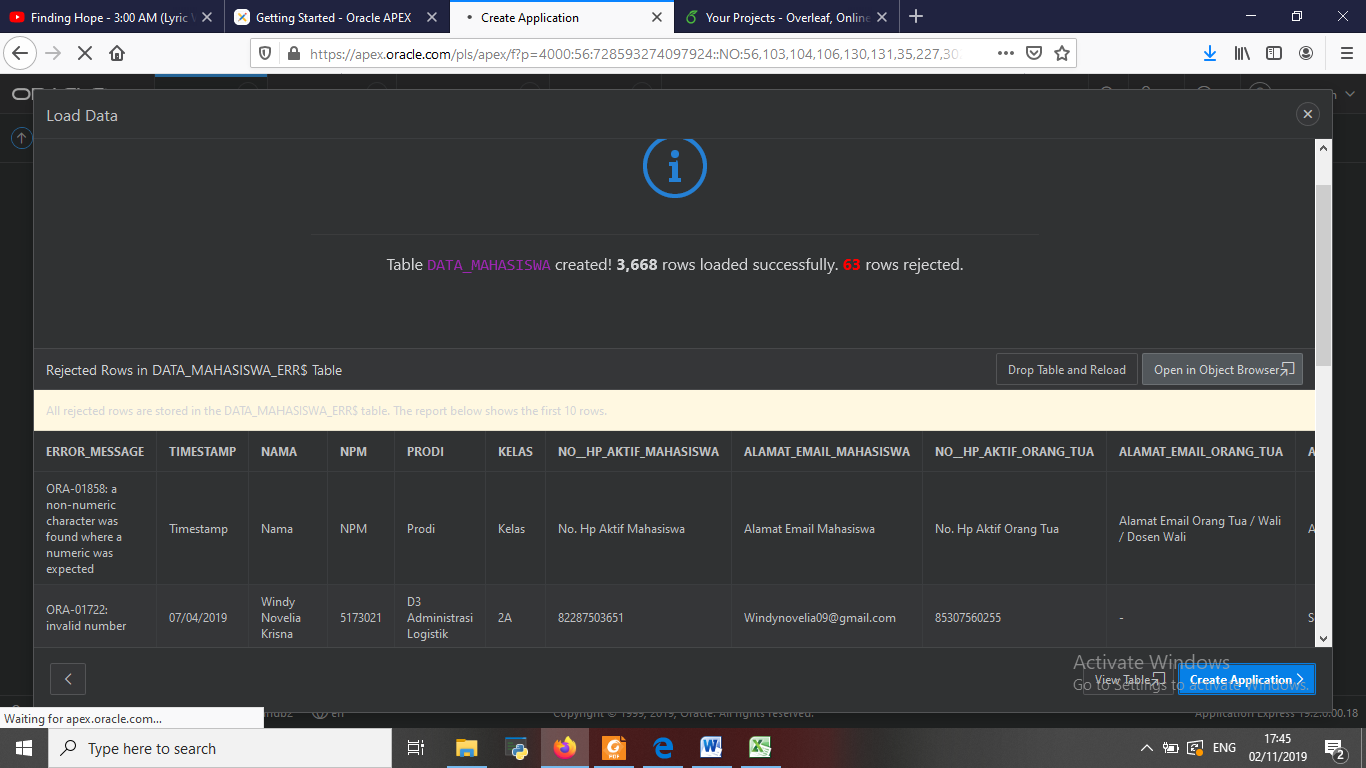
\includegraphics[scale=0.2]{Apex/16.png}
    \end{center}

    \item Kemudian klik Run aplication, dengan memasukan username dan passwordnya
	\begin{center}
    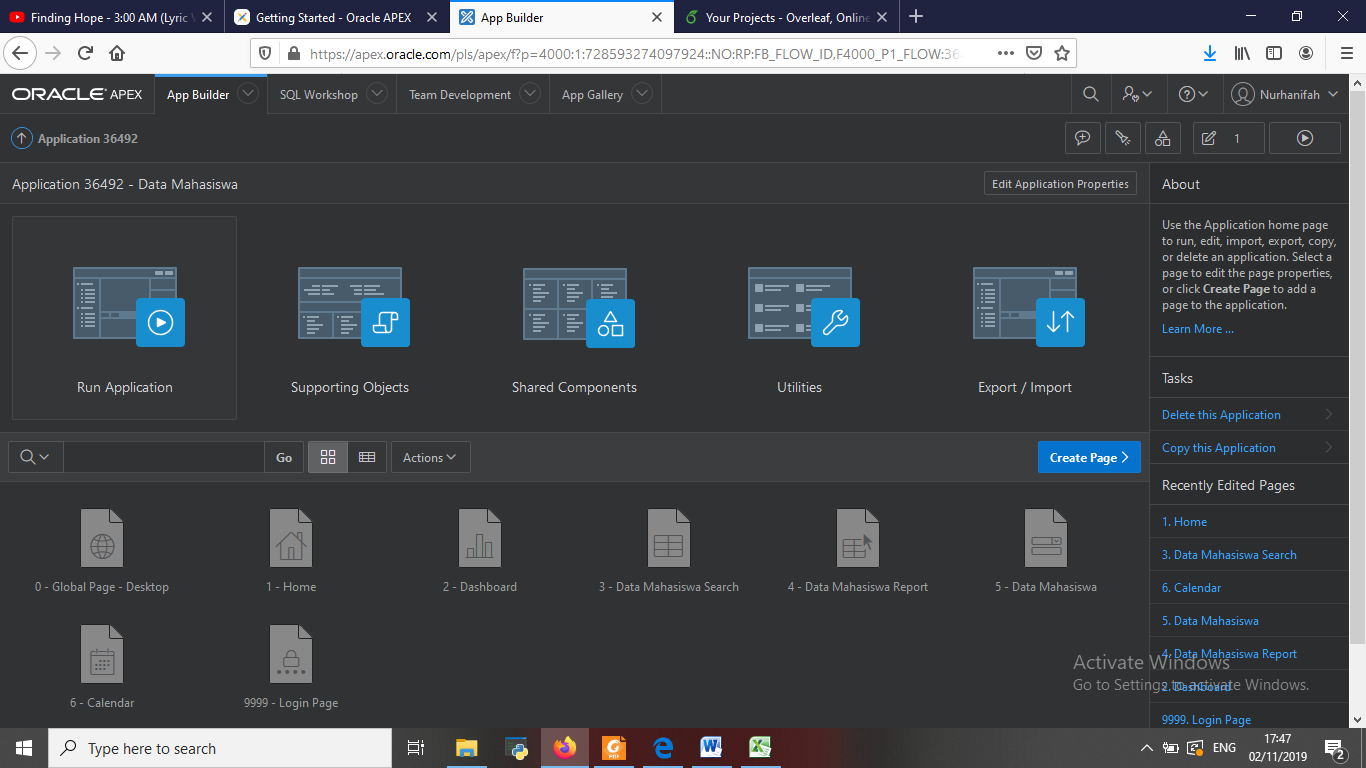
\includegraphics[scale=0.2]{Apex/17.png}
    \end{center}
    
     \item Dan aplication telah selesai dibuat, dapat dilihat seperti gambar dibawah ini
	\begin{center}
    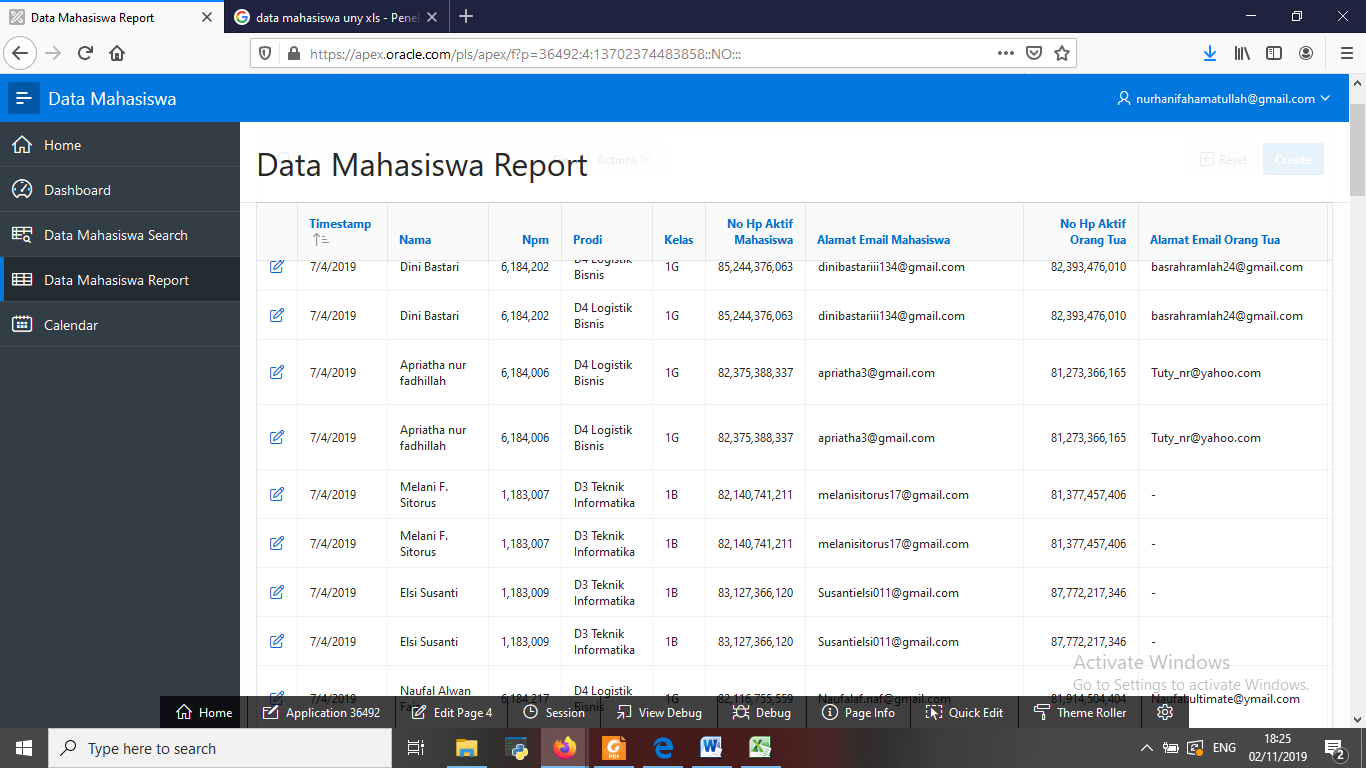
\includegraphics[scale=0.2]{Apex/18.png}
    \end{center}
    
    \item Workspace : LATIHANDB2
    \item USERNAME : nurhanifahamatullah@gmail.com
    \item Password : Hanifah25
     
     

\end{enumerate}
